\setcounter{chapter}{7}
\chapter{Model Analysis}
\label{cha:model_analysis}
% \minitoc
% 
\section{Choise of model parameter}
% 
The goal is to choice a set of parameters, which allow a) fast, b) collision free and c)a high wolume fraction for densly fibers. 
% 
\begin{figure}[!tb]
\centering
\resizebox{1.0\textwidth}{!}{
\def\fiberradius{0.5}
\inputtikz{dev/gfx/2/cube_stat.tex}}
\caption{at fl=3 somethings wrong with the first fr value. Better use time, steps depends on every variable!}
% \label{fig:}
\end{figure}
% 
% \begin{figure}[!tb]
% \centering
% \resizebox{1.0\textwidth}{!}{
% \def\fiberradius{1.0}
% \inputtikz{dev/gfx/2/cube_stat.tex}}
% \caption{at fl=3 somethings wrong with the first fr value. Better use time, steps depends on every variable!}
% % \label{fig:}
% \end{figure}
% % 
% \begin{figure}[!tb]
% \centering
% \resizebox{1.0\textwidth}{!}{
% \def\fiberradius{2.0}
% \inputtikz{dev/gfx/2/cube_stat.tex}}
% \caption{at fl=3 somethings wrong with the first fr value. Better use time, steps depends on every variable!}
% % \label{fig:}
% \end{figure}
% % 
% \begin{figure}[!tb]
% \centering
% \resizebox{1.0\textwidth}{!}{
% \def\fiberradius{5.0}
% \inputtikz{dev/gfx/2/cube_stat.tex}}
% \caption{at fl=3 somethings wrong with the first fr value. Better use time, steps depends on every variable!}
% % \label{fig:}
% \end{figure}
% % 
% \begin{figure}[!tb]
% \centering
% \resizebox{1.0\textwidth}{!}{
% \def\fiberradius{10.0}
% \inputtikz{dev/gfx/2/cube_stat.tex}}
% \caption{at fl=3 somethings wrong with the first fr value. Better use time, steps depends on every variable!}
% % \label{fig:}
% \end{figure}
% 
\section{is overlap important?}
% 
analog analysis like voxelsize
% 
\section{CPU Acceleration}
% 
As described in \dummy \openmp is used for acceleration. This means no usage of multiple computer nodes is currently available. Since the Code traverses an octree, This would not be feasable. Also more then 8 cores \dummy.
% 
\section{Building Models}
% 
\tikzexternaldisable
% 
\begin{figure}[!tb]
\centering
% \resizebox{1.0\textwidth}{!}{
% \inputpdf{dev/gfx/2/cube_2pop_images.pdf}
\begin{tikzpicture}
\node[inner sep=0pt] (image) at (0,0) {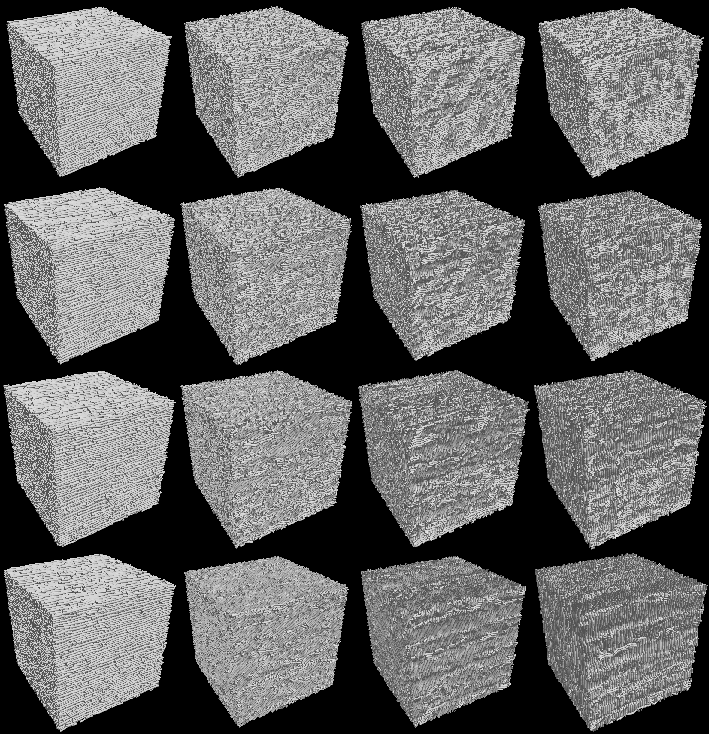
\includegraphics[width=1.0\textwidth, page=1]{dev/gfx/2/cube_2pop_analysis.pdf}};
\begin{scope}[overlay]
    \draw[->,thick] ($(image.north west)-(0.05,-0.05)$) -- ++(1,0) node [midway, above] {$\Omega$};
    \draw[->,thick] ($(image.north west)-(0.05,-0.05)$) -- ++(0,-1) node [midway, above, rotate=90] {$\Psi$};
\end{scope}
\end{tikzpicture}
% }
\caption{}
% \label{fig:}
\end{figure}
% 
% \begin{figure}[!tb]
% \centering
% \resizebox{1.0\textwidth}{!}{
% \begin{tikzpicture}
% \node[inner sep=0pt] (image) at (0,0) {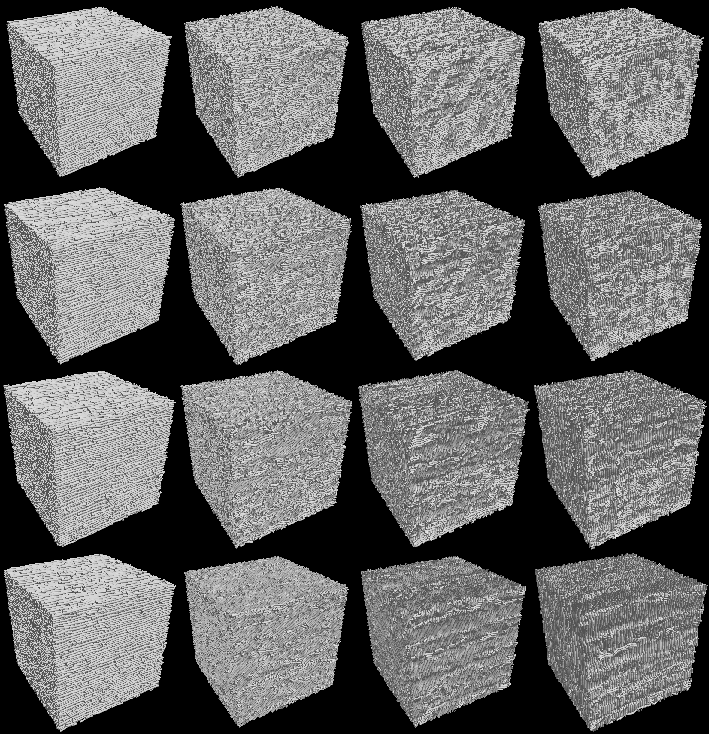
\includegraphics[width=1.0\textwidth, page=1]{dev/gfx/2/cube_2pop_analysis.pdf}};
% \begin{scope}[overlay]
%     \draw[->,thick] ($(image.north west)-(0.25,-0.25)$) -- ++(1,0) node [midway, above] {$\Psi$};
%     \draw[->,thick] ($(image.north west)-(0.25,-0.25)$) -- ++(0,-1) node [midway, above, rotate=90] {$\Omega$};
% \end{scope}
% \end{tikzpicture}
% }
% \caption{}
% % \label{fig:}
% \end{figure}
% 
\tikzexternalenable